% ============================================================
%  Capítulo 5: Resultados preditivos
% ============================================================

\chapter{Resultados preditivos}
\label{cap:resultados_preditivos}

Este capítulo usa o painel do Capítulo~\ref{cap:material} para outra pergunta: quanto tempo de carreira ainda resta a um jogador, dado o retrato da temporada $t$. Vemos como a predição foi avaliada e qual modelo ordena melhor os jogadores. Depois, onde o modelo erra, quem ele aponta como próximo da saída e o que sustenta as suas previsões. Com isso, lemos a lista dos ativos de 2024.

\section{Como a predição foi avaliada}
\label{sec:desenho_aplicado}

O alvo $T$ é o tempo, em anos, entre o fim da temporada $t$ e a saída da liga. A saída segue a definição da Tabela~\ref{tab:decisoes} do Capítulo~\ref{cap:material}, e a censura, a da Seção~\ref{subsec:conceitos_sobrevivencia} do Capítulo~\ref{cap:metodologia}; quem ainda estava na liga em 2024 é censurado. Como o objetivo é prever, cada modelo é testado em temporadas que o ajuste não viu \citep{shmueli2010}, com a validação temporal descrita no Capítulo~\ref{cap:metodologia} (Seção~\ref{sec:validacao_temporal}). Na origem $s$, o treino reúne as temporadas anteriores a $s$, e o teste reúne a temporada $s$. As origens de referência são as de 2018 a 2021. As origens de 2022 e 2023 ficam fora das médias, por terem horizonte de até dois anos. A lista de ativos de 2024 é a aplicação final e não tem desfecho.

Os modelos com covariáveis usam o mesmo conjunto por posição: 25 no QB, 21 no RB e 25 no WR, fixado antes de qualquer origem. Comparamos o Cox com penalização $L_2$, o GBSA e o RSF, e o Kaplan--Meier, sem covariáveis, serve de referência. Em cada origem, os hiperparâmetros são escolhidos só com o treino \citep{varma2006,cawley2010}: os dois últimos anos do treino servem de validação, e a configuração escolhida é reajustada no treino completo antes de ser aplicada ao teste. O treino de cada origem traz só o que se sabia nela (Seção~\ref{subsec:walkforward}). As sensibilidades do protocolo são a borda da grade e a janela de congelamento do X (Apêndice~\ref{sec:busca_aninhada}).

O critério principal é o $C$ de Harrell (Seção~\ref{subsec:cindex}), acompanhado do IBS (Seção~\ref{sec:avaliacao_metodos}). Para o erro em anos, cada modelo prevê a média restrita até $\tau = 2024 - s$, e o erro é medido contra $\min(T,\tau)$. Os contrastes entre modelos são pareados por jogador, com reamostragem \textit{bootstrap} \citep{davison1997}.

O Aalen fica de fora da comparação preditiva. Com as covariáveis dos demais modelos, menos a experiência, que o Aalen não recebe como covariável, a matriz de risco do QB, com 25 colunas, não tem posto completo em nenhum dos 13 tempos de saída da origem de 2018, e um subconjunto menor deixaria de ser comparável aos demais modelos.

\section{Desempenho dos modelos}
\label{sec:bench_wf}

A Figura~\ref{fig:tgb_wf} resume a comparação no \textit{walk-forward}: cada marca colorida é o $C$ de uma origem, e o ponto preto, a média das quatro, com o IC de $95\%$ (valores na Tabela~\ref{tab:tgb_wf}). O $C$ mede a ordenação: é a fração dos pares comparáveis em que o modelo dá maior risco ao jogador que sai antes. Nos três modelos com covariáveis, o $C$ médio fica entre $0{,}661$ e $0{,}709$, contra $0{,}500$ do Kaplan--Meier, que dá o mesmo risco a todos. De cada 100 pares, portanto, os modelos acertam a ordem de 66 a 71, e nenhum intervalo chega a $0{,}50$.

\begin{figure}[H]
\centering
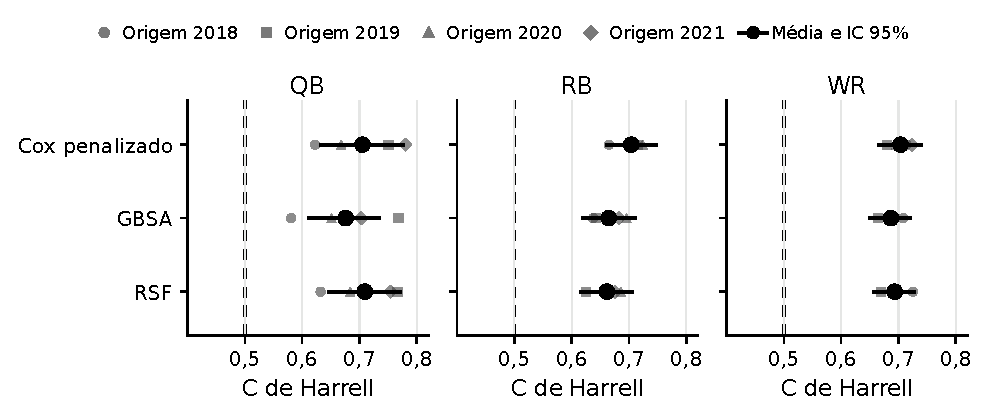
\includegraphics[width=\textwidth,height=0.28\textheight,keepaspectratio]{c_walkforward_folds.pdf}
\caption{C de Harrell por posição e modelo no \textit{walk-forward}. Cada marca colorida é o $C$ de uma origem (2018 a 2021), calculado com todos os pares comparáveis daquela temporada de teste. O ponto preto é a média das quatro origens, e o traço, o IC de 95\% dessa média por \textit{bootstrap} de jogadores ($2\,000$ réplicas): cada réplica sorteia jogadores com reposição e recalcula o $C$ das quatro origens. O intervalo não vem só dos quatro pontos. Tracejado: $C = 0{,}5$, o valor do Kaplan--Meier, que não ordena.}
\label{fig:tgb_wf}
\end{figure}

A figura mostra também que os três modelos ficam próximos, e que só uma vantagem se sustenta. No RB, o Cox fica acima do GBSA e do RSF nas quatro origens, e a diferença para o RSF resiste à correção de Holm nos contrastes pareados ($p$ ajustado de $0{,}016$; Tabela~\ref{tab:tgb_delta}). No QB, RSF e Cox empatam, e só o GBSA fica para trás. No WR, nenhum modelo se separa dos demais. Dentro de cada posição, a diferença de $C$ entre os modelos não passa de $0{,}05$: a forma do modelo pesa menos que a informação do retrato.

Essa informação vai além do tempo de carreira. Um Cox só com a experiência tem $C$ médio entre $0{,}563$ e $0{,}620$, e as demais covariáveis do retrato somam de $0{,}09$ a $0{,}14$ a esse valor. O ganho aparece também na curva prevista, e não só na ordem: o IBS do modelo principal fica de 7\% a 12\% abaixo do Kaplan--Meier nas três posições. E não depende do horizonte desigual das origens: com o desfecho truncado em três anos em todas elas, o $C$ do modelo principal fica entre $0{,}702$ e $0{,}709$.

O modelo usado nas leituras seguintes é o de maior $C$ em cada posição: RSF no QB, Cox no RB e no WR. No RB, a escolha tem apoio do contraste pareado; no QB e no WR, em que os modelos ficam próximos, o maior $C$ decide.

\section{Onde o modelo acerta e onde erra}
\label{sec:acerto_horizonte}

Ordenar bem não garante acertar o prazo. Esta seção mede o erro em anos, verifica em que grupos de risco ele aparece, em que carreiras se concentra e como isso se vê em jogadores concretos.

\subsection{Tamanho do erro e calibração}
\label{sec:calibracao_risco}

A Tabela~\ref{tab:tgb_hit} traz o erro da previsão em anos. Os modelos erram em média cerca de $1{,}3$ ano, pouco menos que o Kaplan--Meier: as covariáveis ajudam mais a ordenar os jogadores do que a acertar o prazo. A média é puxada por uma minoria de erros grandes. A mediana do erro fica abaixo da média em todos os modelos com covariáveis, e cerca de metade das previsões do QB e $40\%$ das do RB e do WR erram por até um ano.

O erro tem direção: os modelos preveem carreira mais longa que a observada, com viés entre $+0{,}28$ e $+0{,}42$ ano nos nove modelos (Tabela~\ref{tab:tgb_hit}). A maior parte desse viés vem da regra de censura, que supõe a saída ao fim da temporada: sem ela, o viés cai para menos de $+0{,}2$ ano (Apêndice~\ref{subsec:apend_censura_pred}). A calibração mostra em que jogadores ele aparece. A Figura~\ref{fig:tgb_calibracao} separa os jogadores em cinco grupos pelo risco que o modelo principal lhes dá, nas origens de 2018 a 2020, e compara a probabilidade prevista de permanecer três anos, $S(3)$, com a observada em cada grupo, estimada por Kaplan--Meier. Na origem de 2021, o acompanhamento termina em três anos, e $S(3)$ não é calculada.

Nela, previsão e observação caem juntas do grupo de menor para o de maior risco, o que confirma a ordenação. A linha, porém, tende a ficar acima das marcas. No RB e no WR, o grupo de menor risco é bem calibrado, e nos demais a permanência prevista supera a observada, em até $0{,}23$. No QB, a diferença chega a $0{,}17$. No RB e no WR, parte dessa distância vem da penalização do Cox, que encolhe os coeficientes e aproxima as previsões da média, efeito que a Seção~\ref{sec:landmark_leitura} mede. Na prática, a ordem entre os grupos é confiável, e a probabilidade é otimista: os grupos de maior risco parecem mais estáveis do que são.

\begin{table}[H]
\centering
\caption{Erro do tempo previsto em anos no \textit{walk-forward}, origens 2018 a 2021: erro absoluto médio (MAE), viés (média de previsto menos observado; positivo indica carreira prevista mais longa que a observada), mediana do erro absoluto e percentual de erro até 1 e 3 anos.}
\label{tab:tgb_hit}
\thesistablesetup\footnotesize
\begin{tabular*}{\textwidth}{@{\extracolsep{\fill}}llccccc@{}}
\toprule
\textbf{Pos.} & \textbf{Modelo} & \textbf{MAE} & \textbf{Viés} & \textbf{Mediana do erro} & \textbf{Erro até 1 ano} & \textbf{Erro até 3 anos} \\
\midrule
QB & Kaplan--Meier & 1{,}48 & $+0{,}18$ & 1{,}26 & 34{,}7\% & 91{,}1\% \\
QB & Cox           & 1{,}30 & $+0{,}30$ & 0{,}94 & 52{,}8\% & 90{,}0\% \\
QB & GBSA          & 1{,}37 & $+0{,}42$ & 1{,}02 & 49{,}4\% & 90{,}4\% \\
QB & RSF           & 1{,}27 & $+0{,}28$ & 0{,}94 & 52{,}0\% & 91{,}1\% \\
\midrule
RB & Kaplan--Meier & 1{,}41 & $+0{,}23$ & 1{,}47 & 38{,}9\% & 95{,}1\% \\
RB & Cox           & 1{,}32 & $+0{,}40$ & 1{,}25 & 40{,}5\% & 97{,}1\% \\
RB & GBSA          & 1{,}38 & $+0{,}39$ & 1{,}24 & 37{,}0\% & 97{,}1\% \\
RB & RSF           & 1{,}29 & $+0{,}33$ & 1{,}18 & 40{,}9\% & 96{,}3\% \\
\midrule
WR & Kaplan--Meier & 1{,}52 & $+0{,}24$ & 1{,}46 & 35{,}9\% & 95{,}1\% \\
WR & Cox           & 1{,}38 & $+0{,}41$ & 1{,}24 & 40{,}3\% & 93{,}7\% \\
WR & GBSA          & 1{,}40 & $+0{,}41$ & 1{,}24 & 39{,}6\% & 93{,}9\% \\
WR & RSF           & 1{,}31 & $+0{,}37$ & 1{,}15 & 44{,}8\% & 95{,}1\% \\
\bottomrule
\end{tabular*}
\end{table}

\begin{figure}[H]
\centering
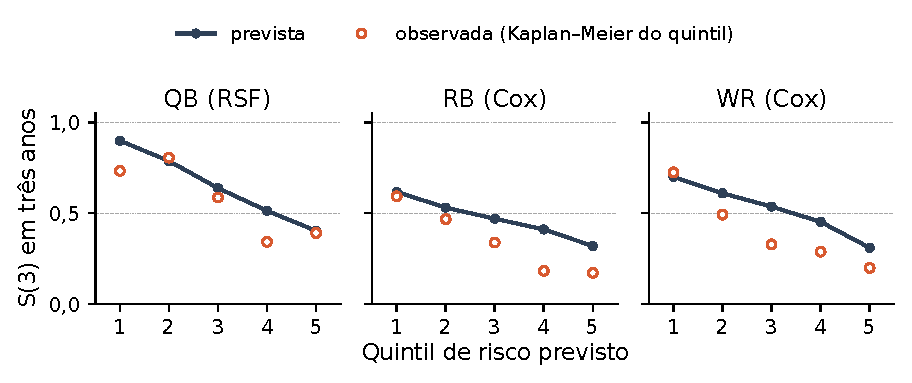
\includegraphics[width=\textwidth]{tgb_calibracao_quintil.pdf}
\caption{Calibração do modelo principal de cada posição no \textit{walk-forward}, origens 2018 a 2020. Os jogadores são divididos em cinco grupos (quintis) pelo risco previsto, do menor (1) ao maior (5). Linha: probabilidade prevista de seguir na liga por mais três anos, $S(3)$, no grupo. Marcas vazadas: a mesma probabilidade observada no grupo, por Kaplan--Meier. Linha acima das marcas indica previsão otimista naquele grupo.}
\label{fig:tgb_calibracao}
\end{figure}

\subsection{Em que carreiras o erro se concentra}
\label{sec:onde_como}

Para ver quem está por trás desse viés, cada par jogador-origem recebe um tipo de trajetória, por regras fixas aplicadas nesta ordem: o par fica com o primeiro tipo cuja regra ele cumpre. \textbf{Além do horizonte}: seguiu na liga até $\tau$, e por isso o erro é negativo por construção, já que a média não passa de $\tau$. \textbf{Hiato}: teve ao menos uma temporada sem jogar entre a primeira e a última da carreira. \textbf{Saída após queda}: a participação ofensiva caiu em duas temporadas seguidas, até a última. \textbf{Saída abrupta}: na última temporada, a participação ofensiva ou a produção da posição estava acima da mediana da posição naquele ano. \textbf{Outras saídas}: as demais. As regras usam o desfecho e a carreira inteira, inclusive os anos posteriores à origem, e servem para mostrar onde o erro cai (Tabela~\ref{tab:tgb_tip}).

\begin{table}[H]
\centering
\caption{Viés médio do modelo principal de cada posição (RSF no QB, Cox no RB e no WR) por tipo de trajetória no \textit{walk-forward}, em anos (previsto menos observado); entre parênteses, o número de pares.}
\label{tab:tgb_tip}
\thesistablesetup
\begin{tabular*}{\textwidth}{@{\extracolsep{\fill}}lccc@{}}
\toprule
\textbf{Tipo} & \textbf{QB} & \textbf{RB} & \textbf{WR} \\
\midrule
Além do horizonte  & $-0{,}84$ (140) & $-1{,}32$ (134) & $-1{,}21$ (266) \\
Hiato              & $+0{,}74$ (62)  & $+0{,}85$ (62)  & $+0{,}68$ (106) \\
Saída após queda   & $+2{,}43$ (14)  & $+0{,}93$ (101) & $+1{,}21$ (127) \\
Saída abrupta      & $+2{,}23$ (27)  & $+1{,}07$ (82)  & $+1{,}58$ (95)  \\
Outras saídas      & $+1{,}85$ (28)  & $+1{,}12$ (132) & $+1{,}43$ (187) \\
\midrule
Todos os pares     & $+0{,}28$ (271) & $+0{,}40$ (511) & $+0{,}41$ (781) \\
\bottomrule
\end{tabular*}
\end{table}

O viés é negativo em quem seguiu além do horizonte e positivo em todos os tipos de saída: quando o jogador sai, o modelo previa mais carreira do que a observada. O erro é maior no QB, perto de dois anos ou mais nos três tipos de saída, e fica perto de um ano no RB e de um ano e meio no WR. O viés não se concentra em um tipo de saída: aparece tanto em quem saiu depois de perder espaço quanto em quem saiu produzindo.

\subsection{Casos no auge}
\label{sec:casos_reais}

A Figura~\ref{fig:tgb_casos} mostra o erro em carreiras concretas do \textit{walk-forward}. São quatro jogadores por posição, todos titulares e entre os dez melhores da posição em jardas na temporada de origem. Em cada linha, as marcas coloridas são os anos previstos pelos três modelos, e o ponto preto, os anos até a saída observada. Os casos foram escolhidos pelo desfecho: ilustram o erro, e não o medem.

A previsão acerta quando o retrato da origem se mantém, e as marcas ficam junto do ponto preto. Kirk Cousins, em 2020, era um titular de 32 anos que quase não perdia jogos: o RSF previu $3{,}9$ anos, e ele seguiu ativo até o fim do horizonte, de quatro anos. Para David Johnson, em 2018, o Cox previu $4{,}1$ anos, e ele saiu após quatro.

O erro típico é a saída que o retrato não anuncia, com as marcas à direita do ponto preto. Philip Rivers, em 2019, tinha 37 anos, 4.615 jardas e nenhum jogo perdido desde 2012: o RSF previu $4{,}4$ anos, e ele jogou só mais uma temporada. Para Leonard Fournette, em 2021, o Cox previu $2{,}4$ anos, e ele saiu após um. São jogadores com produção de quem continua, e é desse tipo de carreira que vem o viés positivo da Tabela~\ref{tab:tgb_tip}. O erro oposto também ocorre: para Mike Evans, em 2018, o Cox previu $4{,}2$ anos, e ele seguia ativo em 2024, além do horizonte de seis anos.

\begin{figure}[H]
\centering
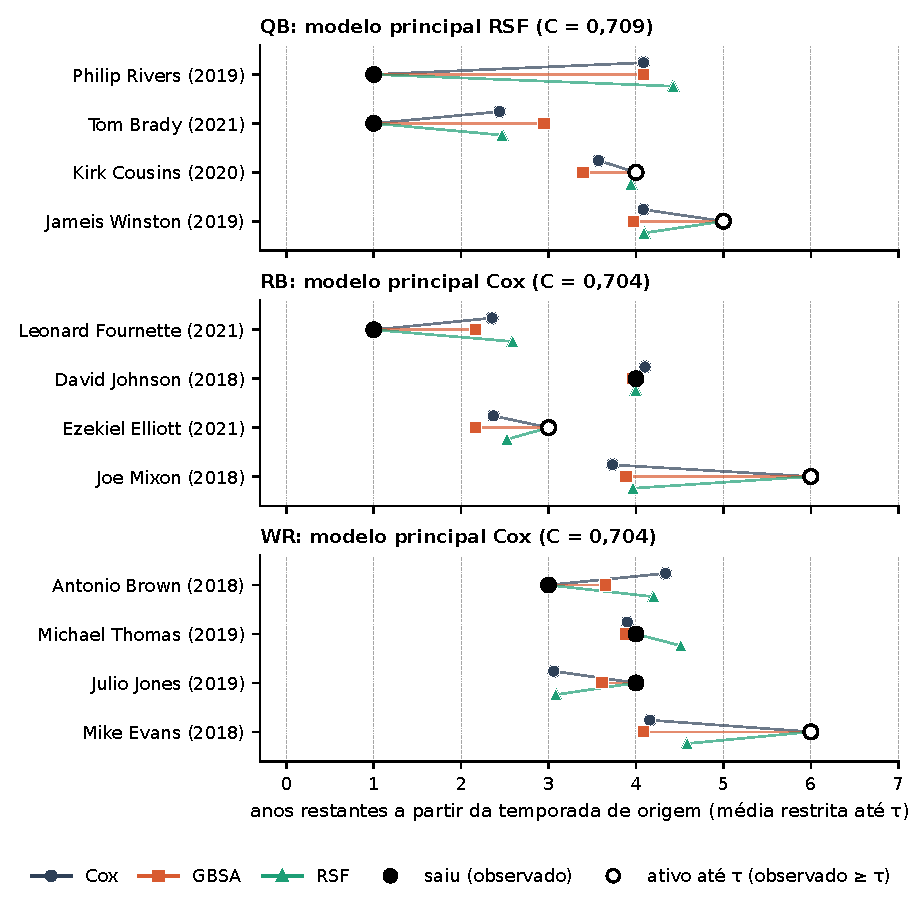
\includegraphics[width=\textwidth,height=0.6\textheight,keepaspectratio]{tgb_casos_leitura.pdf}
\caption{Casos no auge no \textit{walk-forward}, um painel por posição; cada linha é um jogador, com a temporada de origem entre parênteses. Marcas coloridas: anos restantes previstos por Cox (círculo), GBSA (quadrado) e RSF (triângulo). Ponto preto: anos até a saída observada. Círculo vazado: o jogador seguiu ativo até o horizonte $\tau$, então a carreira restante é pelo menos esse valor. O $C$ no título de cada painel é a média do modelo principal no \textit{walk-forward} de 2018 a 2021.}
\label{fig:tgb_casos}
\end{figure}

\section{Quem sai nos próximos anos}
\label{sec:landmark_leitura}

O \textit{walk-forward} responde quanto tempo resta. Para quem decide renovar um contrato por um ou dois anos, a pergunta é outra: entre os jogadores ativos na temporada $s_L$, quem sai da liga nos próximos $w$ anos. É o que o \textit{landmarking} \citep{van_houwelingen2007} mede. Só entram as origens em que a saída em $w$ anos pode ser confirmada, isto é, em que a base cobre a temporada $s_L + w + 1$ (Seção~\ref{subsec:landmarking}): de 2020 a 2022 com $w=1$, 2020 e 2021 com $w=2$ e 2020 com $w=3$. Nessas origens, o $C$ fica entre $0{,}66$ e $0{,}78$ (Apêndice~\ref{sec:ap_landmark}). O desfecho é cortado em $w$, e por isso esse $C$ não se compara ao do \textit{walk-forward}: parte da alta vem do próprio desfecho, mais curto, e parte, do modelo reajustado para o horizonte.

A Figura~\ref{fig:tgb_landmark_quintis} mostra a leitura prática. Dentro de cada origem, os jogadores são repartidos em cinco grupos pelo risco previsto pelo modelo principal, e comparamos, grupo a grupo, a saída prevista e a observada em $w$ anos.

\begin{figure}[H]
\centering
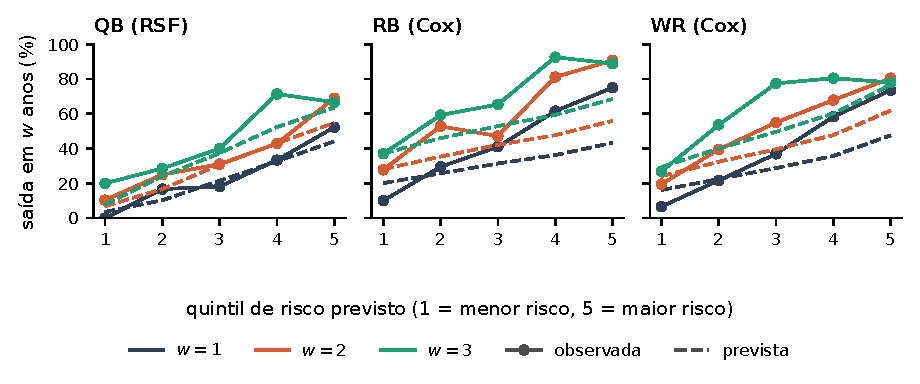
\includegraphics[width=\textwidth,height=0.3\textheight,keepaspectratio]{tgb_landmark_quintis.pdf}
\caption{\textit{Landmarking} com o modelo principal: percentual de saída em $w$ anos por quintil de risco previsto, formado dentro de cada origem (1 = menor risco, 5 = maior). Linha cheia com marcas: saída observada. Linha tracejada: probabilidade média de saída prevista pelo modelo. Cores: horizonte $w$ de 1, 2 e 3 anos.}
\label{fig:tgb_landmark_quintis}
\end{figure}

A saída observada cresce do grupo de menor para o de maior risco, nos três horizontes. Com $w=1$, em que o $C$ é o mais alto (Tabela~\ref{tab:tgb_lm}), saem 52\% dos QBs, 75\% dos RBs e 74\% dos WRs do grupo de maior risco, contra no máximo 10\% no grupo de menor risco. Essa saída soma duas decisões de elenco: não voltar na temporada seguinte, ou jogá-la e não voltar depois. Só a primeira já atinge cerca de metade do grupo de maior risco (45\%, 52\% e 50\%) e quase ninguém no de menor risco. A ordem dada pelo modelo serve, portanto, para separar quem está perto da saída.

A probabilidade prevista é mais tímida que a ordem. No RB e no WR, o Cox comprime os extremos: prevê menos de 50\% de saída no grupo em que cerca de 75\% saem, e prevê mais saída do que ocorre no grupo de menor risco. No QB, o RSF fica mais perto do observado, com 44\% previstos contra 52\%. É o padrão já visto na calibração do \textit{walk-forward} (Seção~\ref{sec:calibracao_risco}), em que o grupo de maior risco parece mais estável do que é, e a penalização $L_2$, que encolhe os coeficientes, explica parte dele no Cox: sem ela, o Cox prevê 55\% e 59\% de saída no grupo de maior risco, sem ganho de $C$. O que se lê com segurança é a posição do jogador entre os grupos, e não a probabilidade.

A origem de 2023 fica fora das médias, porque a saída ao fim de 2024 não pode ser confirmada, mas nela já se sabe quem não voltou em 2024, e os casos repetem o padrão da Seção~\ref{sec:casos_reais}. Os maiores riscos de RB e WR, Brandon Bolden (58\%) e Keith Kirkwood (66\%), vinham de temporadas com dez ou mais jogos perdidos e não jogaram em 2024. Aaron Rodgers, que perdeu 16 jogos em 2023, teve o segundo maior risco entre os QBs (55\%) e voltou. No sentido oposto, Zach Wilson (6\%) era titular e não jogou em 2024, sem que o retrato indicasse isso.

\section{O que sustenta as previsões}
\label{sec:concordancia}

Os três modelos têm formas muito diferentes. Vale, então, perguntar se ordenam os jogadores do mesmo jeito e se usam as mesmas covariáveis para isso.

A Tabela~\ref{tab:tgb_conc} traz a correlação de Spearman entre as previsões de cada par de modelos nas quatro origens do \textit{walk-forward}. Os modelos concordam, e os dois de árvore concordam mais entre si do que com o Cox. Na lista de 2024, em outra população, a correlação fica entre $0{,}88$ e $0{,}98$.

\begin{table}[H]
\centering
\caption{Correlação de Spearman entre as previsões de cada par de modelos no \textit{walk-forward}: média das origens 2018 a 2021.}
\label{tab:tgb_conc}
\thesistablesetup
\begin{tabular*}{\textwidth}{@{\extracolsep{\fill}}lccc@{}}
\toprule
\textbf{Par} & \textbf{QB} & \textbf{RB} & \textbf{WR} \\
\midrule
Cox--GBSA & $0{,}83$ & $0{,}81$ & $0{,}86$ \\
Cox--RSF  & $0{,}88$ & $0{,}86$ & $0{,}89$ \\
GBSA--RSF & $0{,}92$ & $0{,}89$ & $0{,}93$ \\
\bottomrule
\end{tabular*}
\end{table}

A concordância geral esconde desacordos em jogadores específicos. Raheem Mostert, em 2019, é um dos maiores: o GBSA o coloca no percentil 4 do tempo previsto na origem, e o Cox, no percentil 73, mais perto dos cinco anos sem saída que ele teve.

Para ver em que cada modelo se apoia, medimos a queda do $C$ ao permutar cada covariável, que é a medida comparável entre as três famílias. A Tabela~\ref{tab:tgb_imp_inf} traz as covariáveis que ficam entre as cinco primeiras em alguma família, entre as 25 do QB e do WR e as 21 do RB, com a queda no modelo principal.

A ordenação se apoia em poucas covariáveis: no modelo principal, as cinco primeiras respondem por 77\% a 89\% da queda positiva do $C$, e as demais pouco mudam a ordem. O topo tem três temas. O primeiro é o tempo de carreira: a experiência está entre as três mais importantes nas três posições e nos três modelos, como se espera, já que o tempo restante depende do tempo já percorrido.

O segundo tema é o papel na equipe, e o terceiro, a disponibilidade, com peso que muda por posição. No QB, a previsão segue a eficiência e a fatia de passes. No RB, os jogos perdidos ficam em primeiro lugar nos três modelos, seguidos da participação ofensiva. No WR, experiência, jogos perdidos e fatia de alvos se alternam no topo. Os modelos concordam nesse topo e divergem abaixo dele.

\begin{table}[H]
\centering
\caption{Importância por permutação no \textit{walk-forward}: posto em cada modelo (1 = a covariável cuja permutação mais derruba o $C$) e queda do $C$ no modelo principal da posição. Entram as covariáveis que ficam entre as cinco primeiras em algum modelo.}
\label{tab:tgb_imp_inf}
\thesistablesetup
\footnotesize\setlength{\tabcolsep}{3pt}
\begin{tabular*}{\textwidth}{@{\extracolsep{\fill}}llcccc@{}}
\toprule
\textbf{Pos.} & \textbf{Covariável} & \textbf{Cox pen.} & \textbf{GBSA} & \textbf{RSF} & \textbf{Queda do $C$} \\
\midrule
QB & Eficiência de passe (\textit{passer rating}) & 2 & 1 & 1 & $0{,}038$ \\
QB & Fatia de passes da equipe & 3 & 2 & 2 & $0{,}021$ \\
QB & Experiência (anos) & 1 & 3 & 3 & $0{,}015$ \\
QB & Participação ofensiva & 21 & 4 & 4 & $0{,}012$ \\
QB & Profundidade no elenco & 7 & 7 & 5 & $0{,}005$ \\
QB & Hist. defasado jardas por corrida & 5 & 21 & 6 & $0{,}005$ \\
QB & Hiato acumulado na janela & 4 & 6 & 7 & $0{,}004$ \\
QB & Peso & 9 & 5 & 16 & $0{,}000$ \\
\midrule
RB & Jogos perdidos & 1 & 1 & 1 & $0{,}041$ \\
RB & Participação ofensiva & 2 & 2 & 2 & $0{,}026$ \\
RB & Experiência (anos) & 3 & 3 & 3 & $0{,}025$ \\
RB & Fatia de jardas terrestres & 4 & 4 & 4 & $0{,}012$ \\
RB & Hist. defasado YPC & 5 & 6 & 15 & $0{,}010$ \\
RB & Veterano pré-janela & 7 & 5 & 5 & $0{,}006$ \\
\midrule
WR & Experiência (anos) & 1 & 2 & 3 & $0{,}048$ \\
WR & Jogos perdidos & 2 & 3 & 2 & $0{,}045$ \\
WR & Fatia de alvos da equipe & 3 & 1 & 1 & $0{,}021$ \\
WR & Participação ofensiva & 4 & 4 & 4 & $0{,}014$ \\
WR & Veterano pré-janela & 5 & 6 & 5 & $0{,}009$ \\
WR & Hiato acumulado na janela & 6 & 5 & 8 & $0{,}008$ \\
\bottomrule
\end{tabular*}
\end{table}

\section{Aplicação à lista de 2024}
\label{sec:lista_2024}

Com o erro e os sinais conhecidos, a lista de 2024 pode ser lida. Ela reúne os 74 QBs, 107 RBs e 178 WRs ativos naquela temporada e mostra, para cada um, quantos anos de carreira o modelo principal da posição espera: o RSF no QB, e o Cox no RB e no WR, que tiveram o maior $C$ no \textit{walk-forward} de 2018 a 2021. O ajuste segue o mesmo protocolo, com 2024 como origem: o modelo é treinado com as temporadas até 2023 e aplicado ao retrato de 2024. A média é restrita a $\tau = 11$ anos, que é o menor dos maiores seguimentos de treino entre as posições. A base termina em 2024, e a lista não tem desfecho nela: mostra o que o modelo espera de quem estava em campo naquele ano. A Figura~\ref{fig:tgb_lista_2024} mostra os seis maiores e os seis menores valores de cada posição, com a mediana da lista marcada.

No topo estão titulares jovens e produtivos. Entre os QBs, Lamar Jackson, C.J. Stroud e Jalen Hurts estão entre os seis primeiros, que têm de 22 a 29 anos e recebem do RSF entre $8{,}4$ e $9{,}4$ anos, perto do teto de 11. A ponta não é só de quem é novo: Baker Mayfield, com seis anos de carreira, está no mesmo grupo de Stroud, que tem um, porque o modelo lê a produção junto com o tempo já percorrido. Entre os RBs e os WRs, lideram Devon Achane e Malik Nabers, com cerca de sete anos.

No outro extremo estão reservas quase sem participação em 2024, como Josh Johnson, de 38 anos e 16 de carreira, que teve 17 jardas de passe, e WRs que terminaram a temporada sem jardas de recepção.

\begin{figure}[H]
\centering
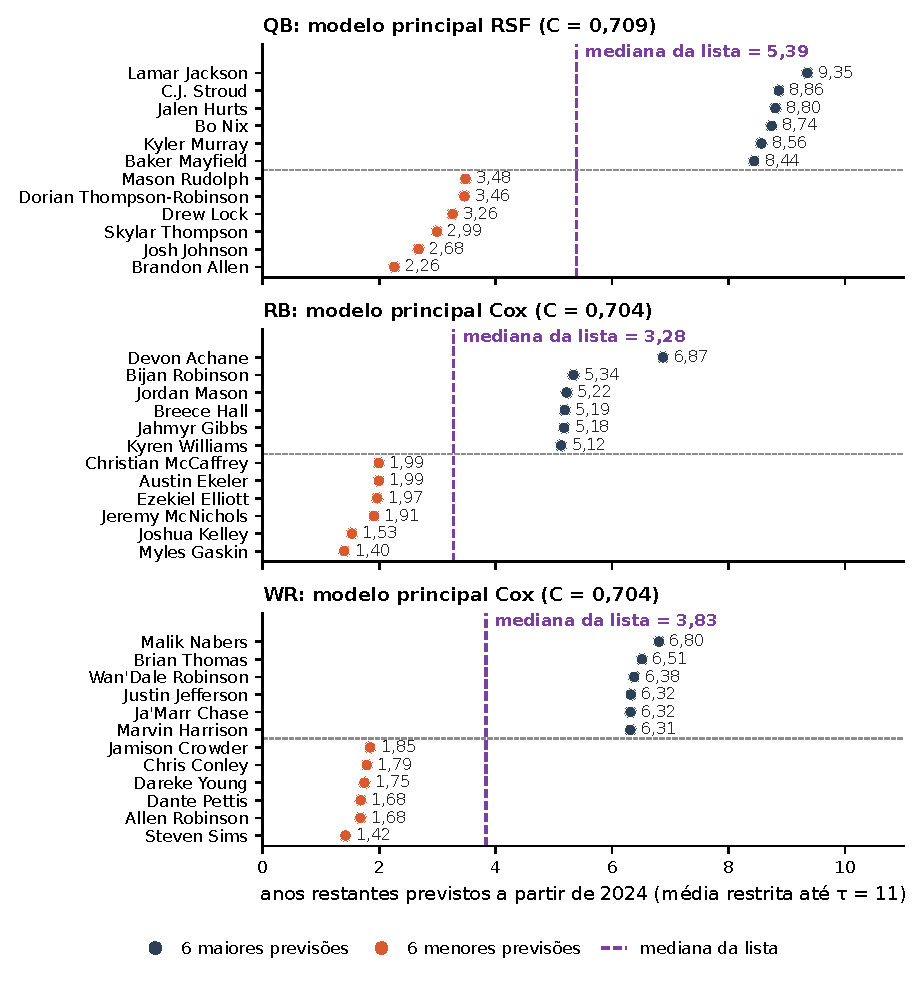
\includegraphics[width=\textwidth,height=0.5\textheight,keepaspectratio]{tgb_lista_2024.pdf}
\caption{Lista de 2024: em cada posição, os seis jogadores com mais anos previstos (azul, acima) e os seis com menos (laranja, abaixo), entre todos os ativos em 2024, pelo modelo principal, treinado com as temporadas até 2023. Previsão: média restrita a 11 anos. Linha tracejada: mediana da lista inteira da posição. O $C$ no título de cada painel é a média do \textit{walk-forward} de 2018 a 2021; a lista não tem desfecho e, por isso, não tem $C$ próprio.}
\label{fig:tgb_lista_2024}
\end{figure}

A Figura~\ref{fig:tgb_lista_quintis} olha a lista inteira, e não só os extremos: os ativos de 2024 são divididos em cinco grupos pelo risco que o modelo principal lhes dá. Do grupo de menor risco para o de maior, a fatia da equipe e a participação ofensiva caem e os jogos perdidos sobem, nas três posições. No QB, por exemplo, a mediana da fatia de passes vai de $0{,}89$ a $0{,}06$. A experiência não segue um padrão único: no RB e no WR, o grupo de maior risco reúne jogadores mais experientes, e no QB a curva oscila. A previsão se apoia, assim, nos mesmos temas da Seção~\ref{sec:concordancia}: o papel na equipe e a disponibilidade.

\begin{figure}[H]
\centering
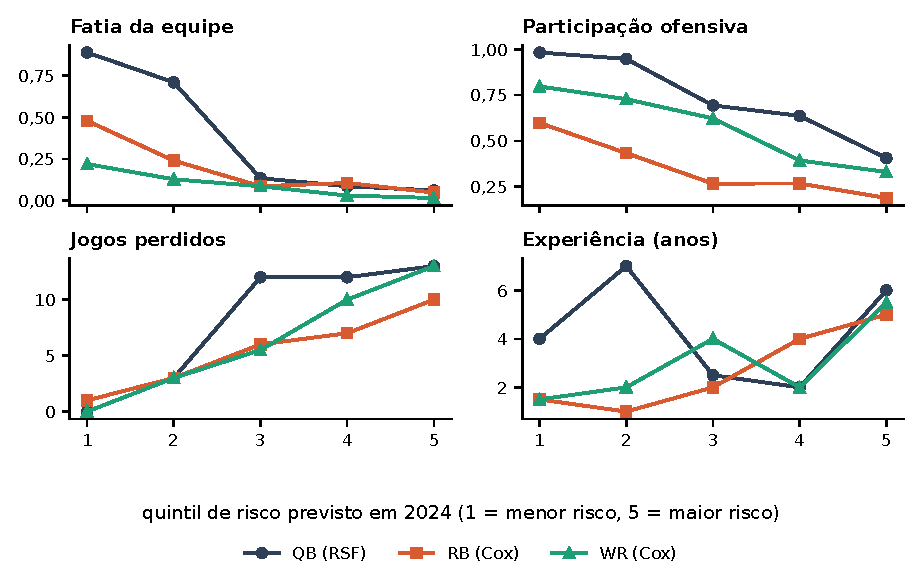
\includegraphics[width=\textwidth,height=0.32\textheight,keepaspectratio]{tgb_lista_quintis.pdf}
\caption{Lista de 2024 por quintil de risco previsto pelo modelo principal (a mesma previsão da Figura~\ref{fig:tgb_lista_2024}): 1 reúne os jogadores com mais anos previstos (menor risco) e 5, os com menos (maior risco). Cada ponto é a mediana do grupo, com todos os ativos de 2024 (cerca de 15 jogadores por grupo no QB, 21 no RB e 36 no WR). Fatia da equipe e participação ofensiva vão de 0 a 1.}
\label{fig:tgb_lista_quintis}
\end{figure}

O erro foi medido com horizontes de 3 a 6 anos, e a lista vai a 11: os anos acima de seis são extrapolação do modelo, e a lista vale pela ordem que dá aos jogadores.

Os modelos nem sempre concordam sobre um jogador: Amon-Ra St. Brown é o 8º WR no Cox e o 20º no GBSA. A lista mede tempo de carreira esperado, não qualidade atual. O que esses sinais significam em risco, e até onde coincidem com a inferência, é o tema do Capítulo~\ref{cap:discussao}.

